\chapter{PROBLEM}

\section{Problem}
The basic problem in this thesis is how to find appropriate job descriptions by user's r\'esum\'e. If we take the r\'esum\'e as a query and the job descriptions as documents, we need to build an information retrieval model to get the most relevance documents.  The JobFinder will parse the job descriptions to the job models, and store them in the database. When a user searches the jobs by their r\'esum\'e in the system, the system will compare the similarity values between the r\'esum\'e and the job models, and return the jobs sorted by their similarity values.

The core idea of our algorithm is calculate similarity between the r\'esum\'e model and job model.
We give a formal definition of our problem. All of the notations will be used frequently throughout the thesis.

We use $r$ to denote the user's r\'esum\'e model, which has some features $r_i$ like their academic degree, their major, their skills and so on. The symbol $J$ is the set of job models stored in the database, and $j$ is a job model in the set $J$. The similarity function $sim(r, j)$ gives the similarity values between r\'esum\'e $r$ and job $j$. The return list of search function $search(r,J)$ will calculate all the similarity value in the database, and the result of the function will be the job description list ranked by their similarity values. The equation of how to calculate similarity value is given below:

$$ sim(r, j) = \sum_{i=1}^{n} simfun_i(r_i,j_i) \times w_i $$

The value of $sim(r, j)$ is the summation of the similarity values of different fields times their corresponding weights. Different fields like major and skills,  may have different functions to calculate their similarity values. We will describe the similarity functions of individual fields in later parts.


\section{Model Similairty}

In our system, the r\'esum\'e model and job model both have four fields: job title, major, academic degree and skills. The similarity value between a r\'esum\'e model and job model is the sum of the similarity values of all the fields pairs time their weights. We will introduce how to calculate similarity value for each field in the chapter.

\subsection{Major and Academic Degree}

In the simplest case, if the majors in the r\'esum\'e model and job model are same, the similarity value is 1. If they are different, we can check whether the major in the r\'esum\'e model is in the list of related majors of the major in the job model. If it is, the similarity value is 0.5, otherwise the similarity value is 0.

The are five academic degree types in the system:  high school degree, associate degree, bachelor degree, master degree, and Ph.D. degree, which are mapped to the integer value form 1 to 5. If the degree value in the r\'esum\'e model is less than that in the job model, which means that the job seeker's education background cannot satisfy the requirement of the job, the similarity value in this case is 0. If the degree value in the r\'esum\'e model is equal or no more than 2 bigger than that of the job model, the similarity value is 1. In some cases, the degree value in the r\'esum\'e model is greater than that of the job model, and the difference is greater than 2, which means the job seeker's degree is much higher than the requirement of the job. In such case, the similarity value is given 0.5. The system combines the similarity values of major and degree together by return the product of them.

$$ Sim(p1, p2) = \begin{Bmatrix}
1, & if~similarity~of~p1~and~p2 \geqslant t\\
0, & otherwise
\end{Bmatrix} $$

\subsection{Job Title}

A job title can be parsed into some sub fields: job type, level, platform, programming language, and so on.  The value of job type includes: developer, manager, administrator and so on. The levels values are junior, senior, architect, and so on. The platforms include: web, mobile, cloud and so on. If the job seeker has some working experience, there should be some job titles in their resume.  When calculating the similarity value between a r\'esum\'e model and a job model, the system calculates the similarity values of the title of job model to all the titles in the r\'esum\'e model, and return the maximum one.


\chapter{System Overview}

\section{System Overview}
The system uses a rule based information extraction technique to parse job descriptions and r\'esum\'es, and gets information such as skills, specialties and education background. The information is used to create the models of job openings and job seekers. A domain specific ontology is used to construct the knowledge base, which includes the taxonomies that support r\'esum\'e-job matching.

The models of r\'esum\'e includes job seekers' specialties, working experience and education background, and all the fields are extracted from their r\'esum\'es. The job models are extracted from job descriptions, and have the same information fields as the r\'esum\'e models.  When a job seeker searches the jobs by their r\'esum\'e, the system calculates the similarity between the candidate model and job models, then gives every job model a similarity score.

\section{System Architecture}

Figure~\ref{fig:Pipeline} shows the architecture of the whole system, which includes such modules:

\begin{enumerate}
    \item The web scrawler can access and download all new IT job opening web pages from indeed.com everyday.
    \item Job parser can parse the job opening web pages, extract the information and create the job models.
    \item Resume Parser is much like the Job parser, it parses the r\'esum\'es and create the r\'esum\'e models.
    \item All the job descriptions and job models are stored in the database.
    \item When a user searches  the jobs with their r\'esum\'e, the ontology matcher calculates the similarity scores of jobs in the database, and returns the jobs ranked by their similarity scores.
\end{enumerate}

\begin{figure}[htbp]
  \centering
  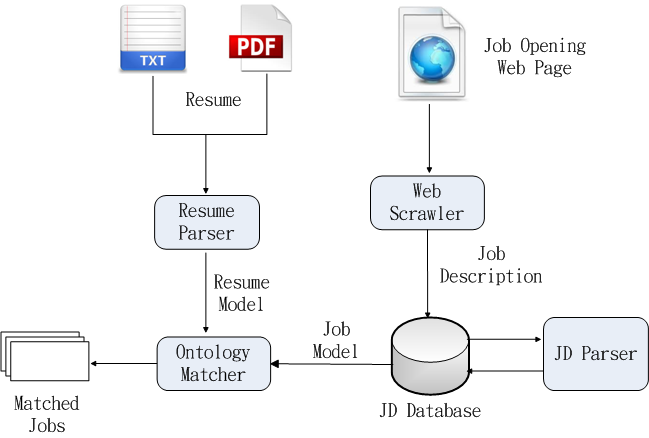
\includegraphics[scale=0.5]{images/arch.png}
  \caption{System Architecture}
  \label{fig:arch}
\end{figure}

\section{System Implementation}

We will describe some implementation details here. The whole system is implemented in Python, and uses some third party libraries and frameworks. We used Flask, a lightweight web framework, to build the web application. We used Rdflib as the OWL file parser, PLY(Python Lex-Yacc) as the token regular expression compiler, whoosh as the unversed index builder and Beautiful Soup as the HTML parser.  All the jobs got by the web crawler are stored in the MongoDB NoSQL database.  For the natural language processing part, we used Natural Language Toolkit (NLTK), a  natural language processing library, to extract the sentences and tokenized them.

\section{System Interface}

The system provide some interfaces to end users. The most important interfaces include the web pages reviewing all the jobs in the database, searching the jobs by keyword Figure~\ref{fig:joblist},  uploading user's r\'esum\'e ~\ref{fig:upload_resume},  matching the jobs with r\'esum\'e~\ref{fig:match_resume} and searching the jobs with both keyword and r\'esum\'e~\ref{fig:keyword_resume}.

\begin{figure}[htbp]
  \centering
  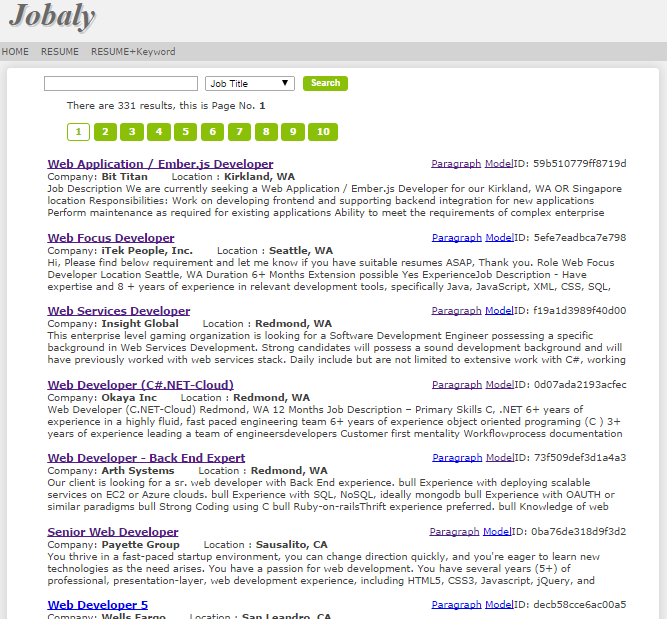
\includegraphics[scale=0.5]{images/joblist.png}
  \caption{Job Description List}
  \label{fig:joblist}
\end{figure}


\begin{figure}[htbp]
  \centering
  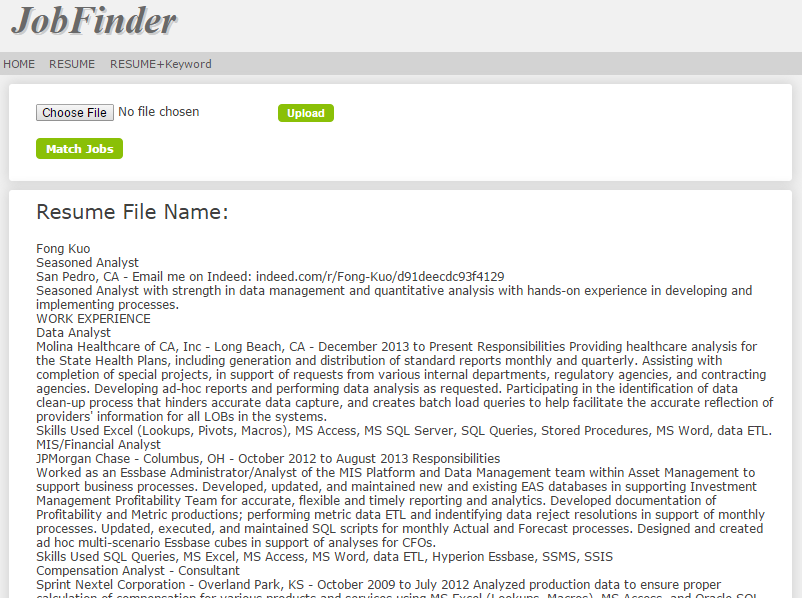
\includegraphics[scale=0.5]{images/upload_resume.png}
  \caption{Upload Resume}
  \label{fig:upload_resume}
\end{figure}

\begin{figure}[htbp]
  \centering
  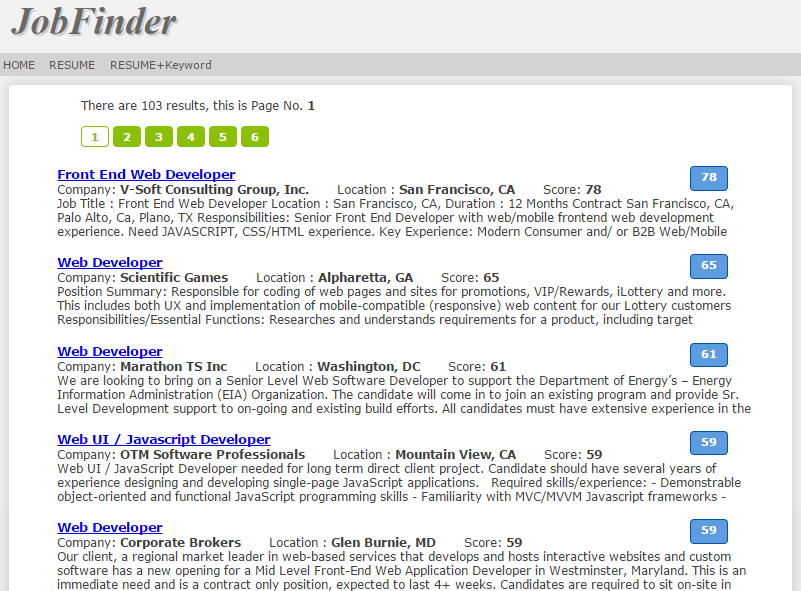
\includegraphics[scale=0.5]{images/match_resume.png}
  \caption{Resume Job matching }
  \label{fig:match_resume}
\end{figure}

\begin{figure}[htbp]
  \centering
  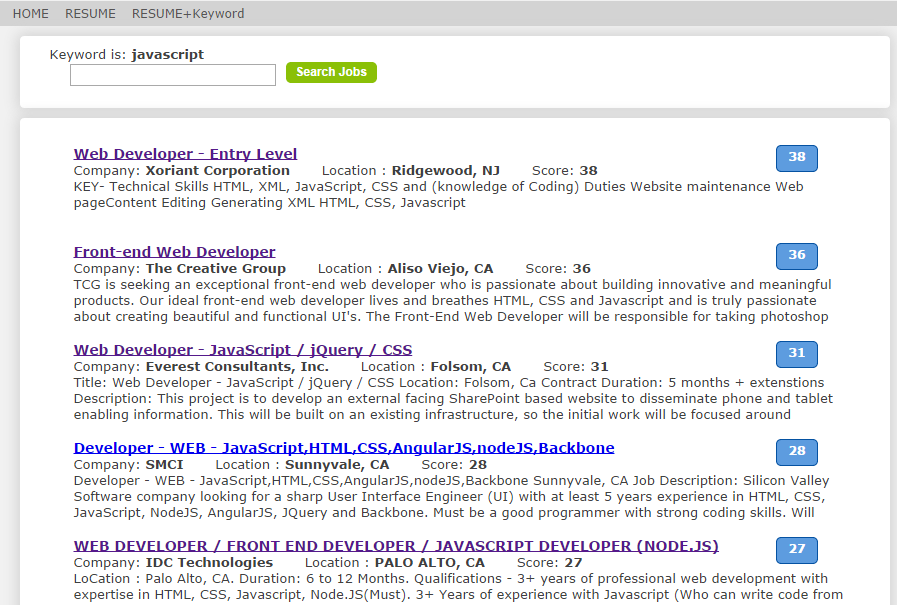
\includegraphics[scale=0.5]{images/keyword_resume.png}
  \caption{Combine the Keyword and Resume Matching}
  \label{fig:keyword_resume}
\end{figure}






